\documentclass{article}
% 如果没有这一句命令,XeTeX会出错,原因参见
% http://bbs.ctex.org/viewthread.php?tid=60547
% \DeclareRobustCommand\nobreakspace{\leavevmode\nobreak\ }
%%%%%%%%%%%%%%%%%+++++++++++
\usepackage{eso-pic} 
% This package makes it easy to add some picture commands to every page at ab-solute positions
\usepackage{hyperref,graphicx,xcolor} %超链接,图形包,图片
%\definecolor{ocre}{RGB}{243,102,25} %定义一个颜色
% xcolor package starts from the basic facilities of the 
% color package, and provides easy driver-independent access
%to several kinds of color tints, shades, tones, 
%and mixes of arbitrary colors
\usepackage{amsmath,amssymb,amsfonts} % 数学字体
\usepackage{mathrsfs} % 提供了mathscr 命令
% Required for specifying colors by name 
\usepackage{enumerate} 

\usepackage{hepunits} % hep units
\usepackage{braket} % Dirac bra-ket notation% useful for Feynman slash notation
\usepackage{slashed} % also for slash notation: take your pick!
\usepackage{bm,bbm} 
%\bm which makes its argument bold
%Blackboard variants of Computer Modern fonts.
\usepackage{simplewick} 
% a simple means of drawing Wick contractions above and below expressions. 
\usepackage{makeidx} 
% Standard package for creating indexes
\usepackage{multirow}
\usepackage{mathtools}% 定义配对的数学符号
\DeclarePairedDelimiter\abs{\lvert}{\rvert}
%%\usepackage[colorlinks,linkcolor=blue]{hyperref} 
\usepackage{tikz-feynman}  % 画费曼图用
\usepackage{tikz}
%%++++++++++++++++++++ 
\DeclareMathOperator{\tr}{Tr}
%\DeclareMathOperator{\re}{Re}
%\DeclareMathOperator{\im}{Im}
\DeclareMathOperator{\res}{Res}
\DeclareMathOperator{\disc}{Disc}
\newcommand*{\dif}{\mathop{}\!\mathrm{d}}
\newcommand{\cola}[1]{{\color{blue}{#1}}}
%%%+++++++++++++++++++++++++++++++
\usepackage{listings}
% 在LaTex中添加代码高亮
\usepackage{framed}
% 在对象周围添加方框,阴影等等,允许跨页
\definecolor{shadecolor}{rgb}{0.9,0.9,0.9}
%定义各种颜色
\definecolor{codegreen}{rgb}{0,0.6,0}
\definecolor{codegray}{rgb}{0.5,0.5,0.5}
\definecolor{codepurple}{rgb}{0.58,0,0.82}
\definecolor{backcolour}{rgb}{0.95,0.95,0.92}
%\lstdefinestyle{〈style name〉}{〈key=value list〉}
%stores the key=value list
\lstdefinestyle{codestyle1}{
    backgroundcolor=\color{backcolour},   
    commentstyle=\color{codegreen},
    keywordstyle=\color{magenta},
    numberstyle=\tiny\color{codegray},
    stringstyle=\color{codepurple},
    basicstyle=\footnotesize,
    breakatwhitespace=false,         
    breaklines=true,                 
    captionpos=b,                    
    keepspaces=true,                 
    numbers=left,                    
    numbersep=5pt,                  
    showspaces=false,                
    showstringspaces=false,
    showtabs=false,                  
    tabsize=2
}



\usepackage{kantlipsum}

\usepackage{fontspec}
\usepackage{unicode-math}
\setmainfont{lmroman10-regular.otf}
\setmathfont{latinmodern-math.otf}

\begin{document}

\begin{align}
    &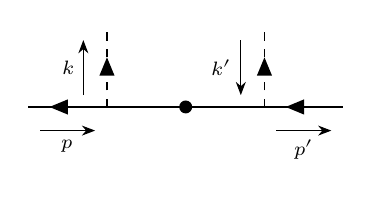
\begin{tikzpicture}[baseline]
        \begin{feynman}
            %% fig a
            \vertex (a1) at (0,0);
            \vertex[right =1cm  of a1] (a2);
            \vertex[right =2cm  of a1,dot,anchor=center] (a3){};
            \vertex[right =3cm  of a1] (a4);
            \vertex[right =4cm  of a1] (a5);
            \vertex[above =1cm of a2] (a6);
            \vertex[above =1cm of a4] (a7);
            %\node[above =1.5cm  of a5] {$a$};
            \diagram*{
            { [edge=anti fermion]
                    (a1) --[momentum'={\scriptsize \(p\)}]  (a2),
                    (a4) --[momentum'={\scriptsize \(p^{\prime}\)}]  (a5),
                },
                % 介子连线
            { [edge= charged scalar]
            (a2) --[momentum={\scriptsize \(k\)}](a6), 
            (a4) --[reversed momentum={\scriptsize \(k^{\prime}\)}](a7), 
            },
            (a2) --  (a4),
            };
        \end{feynman}
    \end{tikzpicture}
    =\slashed{k}^{\prime}\gamma^{5}\cdots\gamma^{5}\slashed{k} \\
    &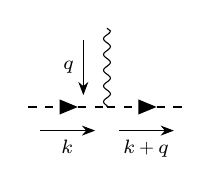
\begin{tikzpicture}[baseline]
        \begin{feynman}
                %% fig a
                \vertex (a1) at (0,0);
                \vertex[right =1cm  of a1] (a2);
                \vertex[right =2cm  of a1] (a3);
                \vertex[right =3cm  of a1] (a4);
                \vertex[right =4cm  of a1] (a5);
                \vertex[above =1cm of a2] (a6);
                \vertex[above =1cm of a4] (a7);
                %\node[above =1.5cm  of a5] {$a$};
                \diagram*{
                { [edge = charged scalar ]
                        (a1) --[momentum'={\scriptsize \(k\)}]  (a2),
                        (a2) -- [momentum'={\scriptsize \(k+q\)}] (a3),
                },
                 % 介子连线
                { [ edge= photon]
                (a2) --[reversed momentum = {\scriptsize \(q\)}](a6), 
                }
                };
            \end{feynman}
        \end{tikzpicture}
    =\left(+i\right)i\left(k+k+q\right)^{\mu}=-\left(k+k+q\right)^{\mu}
    \end{align}

\end{document}



